% !TEX root = ../Main.tex

\subsection{Atomistix ToolKit: ATKPython and Nanolanguage}
In this project we will utilise the Atomistix ToolKit, developed by QuantumWise A/S\cite{QuantumWise}, or ATK for short. The Toolkit takes Python scripts as inputs and simulates a completely custom lattice enviroment with various applied calculations. It is possible to simulate very specific scenarios, alter the simulation parameters and extract results for analysis easily and fast.
ATKPython (the standalone simulation program) extends the Python language with Nanolanguage which tells ATKPython what to do when launched. One can set up specific bravais lattices and repeat them into large 2D structures. Then specific atoms can be tagged or altered and calculations can be set up. All of these features are available through QuantumWise VNL, a GUI which sets up the scripts and calculations, if need be. When working with VNL both the GUI and the CLI are used. In our case, the GUI serves mostly as a visual aid for understanding the modes with 3D graphics and easy graph extraction. The typical workflow when using VNL and ATK is depicted on \cref{workflow}
\begin{figure}
  \centering
  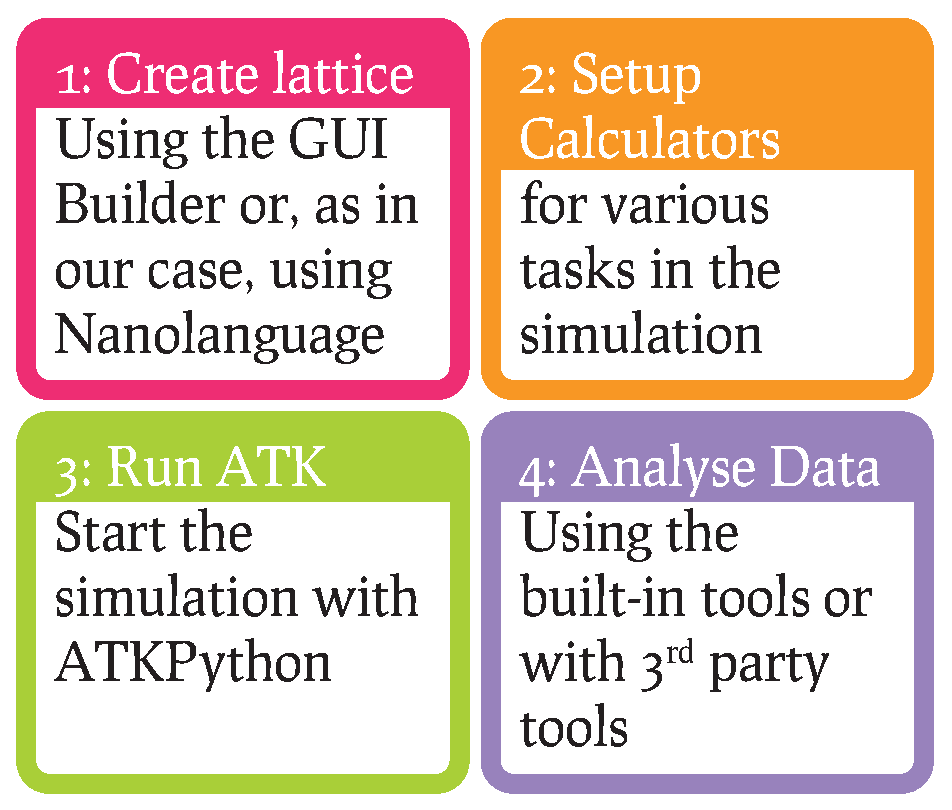
\includegraphics[width=\columnwidth]{Figures/Workflow.eps}
  \caption{Diagram showing the typical workflow in VNL.}
  \label{workflow}
\end{figure}
